\documentclass{article}\usepackage[]{graphicx}\usepackage[]{color}
%% maxwidth is the original width if it is less than linewidth
%% otherwise use linewidth (to make sure the graphics do not exceed the margin)
\makeatletter
\def\maxwidth{ %
  \ifdim\Gin@nat@width>\linewidth
    \linewidth
  \else
    \Gin@nat@width
  \fi
}
\makeatother

\definecolor{fgcolor}{rgb}{0.345, 0.345, 0.345}
\newcommand{\hlnum}[1]{\textcolor[rgb]{0.686,0.059,0.569}{#1}}%
\newcommand{\hlstr}[1]{\textcolor[rgb]{0.192,0.494,0.8}{#1}}%
\newcommand{\hlcom}[1]{\textcolor[rgb]{0.678,0.584,0.686}{\textit{#1}}}%
\newcommand{\hlopt}[1]{\textcolor[rgb]{0,0,0}{#1}}%
\newcommand{\hlstd}[1]{\textcolor[rgb]{0.345,0.345,0.345}{#1}}%
\newcommand{\hlkwa}[1]{\textcolor[rgb]{0.161,0.373,0.58}{\textbf{#1}}}%
\newcommand{\hlkwb}[1]{\textcolor[rgb]{0.69,0.353,0.396}{#1}}%
\newcommand{\hlkwc}[1]{\textcolor[rgb]{0.333,0.667,0.333}{#1}}%
\newcommand{\hlkwd}[1]{\textcolor[rgb]{0.737,0.353,0.396}{\textbf{#1}}}%
\let\hlipl\hlkwb

\usepackage{framed}
\makeatletter
\newenvironment{kframe}{%
 \def\at@end@of@kframe{}%
 \ifinner\ifhmode%
  \def\at@end@of@kframe{\end{minipage}}%
  \begin{minipage}{\columnwidth}%
 \fi\fi%
 \def\FrameCommand##1{\hskip\@totalleftmargin \hskip-\fboxsep
 \colorbox{shadecolor}{##1}\hskip-\fboxsep
     % There is no \\@totalrightmargin, so:
     \hskip-\linewidth \hskip-\@totalleftmargin \hskip\columnwidth}%
 \MakeFramed {\advance\hsize-\width
   \@totalleftmargin\z@ \linewidth\hsize
   \@setminipage}}%
 {\par\unskip\endMakeFramed%
 \at@end@of@kframe}
\makeatother

\definecolor{shadecolor}{rgb}{.97, .97, .97}
\definecolor{messagecolor}{rgb}{0, 0, 0}
\definecolor{warningcolor}{rgb}{1, 0, 1}
\definecolor{errorcolor}{rgb}{1, 0, 0}
\newenvironment{knitrout}{}{} % an empty environment to be redefined in TeX

\usepackage{alltt}
\title{Mental Health Survey Analysis}
\author{Tommy Carpenito and Lina Montoya}
\date{\today}


\usepackage{float}
\usepackage{amsmath}
\usepackage[top=1in, bottom=1.5in, left=.5in, right=.5in]{geometry}
\usepackage{rotating}
\IfFileExists{upquote.sty}{\usepackage{upquote}}{}
\begin{document}
\maketitle
\tableofcontents

\pagebreak

\section{Demographics}
The following section compares the ethnic diversity of the Fall 2016 undergraduates at the University of California, Berkeley (UCB) with the profile of survey participants who completed the ``Undergraduate Student Well-being Survey - 2016" (USWBS), as populated by the UCB.
\subsection{UC Berkeley Demographics}

\begin{kframe}


{\ttfamily\noindent\itshape\color{messagecolor}{\#\# \\\#\# Attaching package: 'gplots'}}

{\ttfamily\noindent\itshape\color{messagecolor}{\#\# The following object is masked from 'package:stats':\\\#\# \\\#\#\ \ \ \  lowess}}\end{kframe}% latex table generated in R 3.3.1 by xtable 1.8-2 package
% Sat Feb  4 14:12:22 2017
\begin{table}[ht]
\centering
\begin{tabular}{lrrrrr}
  \hline
Ethnicity & Count & Prop. Female & Prop. Male & Prop. Undefined & Prop. Total \\ 
  \hline
African American/Black & 947 & 0.58 & 0.41 & 0.00 & 0.03 \\ 
  Mexican American/Chicano & 3056 & 0.59 & 0.41 & 0.00 & 0.10 \\ 
  Other Hispanic/Latino & 1102 & 0.57 & 0.43 & 0.00 & 0.04 \\ 
  Native American/Alaska Native & 172 & 0.58 & 0.41 & 0.01 & 0.01 \\ 
  Pacific Islander &  58 & 0.57 & 0.43 & 0.00 & 0.00 \\ 
  Chinese & 5050 & 0.51 & 0.48 & 0.00 & 0.17 \\ 
  Filipino & 867 & 0.59 & 0.41 & 0.00 & 0.03 \\ 
  Japanese & 461 & 0.57 & 0.43 & 0.00 & 0.02 \\ 
  Korean & 1347 & 0.49 & 0.51 & 0.00 & 0.05 \\ 
  Other Asian & 331 & 0.57 & 0.43 & 0.00 & 0.01 \\ 
  South Asian & 2240 & 0.46 & 0.53 & 0.00 & 0.08 \\ 
  Vietnamese & 907 & 0.58 & 0.42 & 0.00 & 0.03 \\ 
  White & 7594 & 0.50 & 0.50 & 0.00 & 0.26 \\ 
  Decline to State & 1199 & 0.42 & 0.42 & 0.16 & 0.04 \\ 
  International & 3979 & 0.49 & 0.50 & 0.01 & 0.14 \\ 
  Total & 29310 & 0.52 & 0.47 & 0.01 & 1.00 \\ 
  Underrepresented Minority Subtotal & 5277 & 0.58 & 0.41 & 0.00 & 0.18 \\ 
   \hline
\end{tabular}
\caption{Data representing the ethnic diversity of the Fall 2016 undergradates at UCB. Information provided from the office of planning and development  (http://opa.berkeley.edu/uc-berkeley-fall-enrollment-data).} 
\end{table}


This table was made in order to make a comparison with the survey demographics (Table 2). Note: underrepresented groups are defined as African American, Chicano/Latino, and Native American/Alaska Native.

\pagebreak

\subsection{Survey Demographics}
 
% latex table generated in R 3.3.1 by xtable 1.8-2 package
% Sat Feb  4 14:12:22 2017
\begin{table}[ht]
\centering
\begin{tabular}{lrr}
  \hline
Ethnicity & Count & Proportion \\ 
  \hline
                         White & 156 & 0.1692 \\ 
                          Korean & 21 & 0.0228 \\ 
                         Chinese & 115 & 0.1247 \\ 
                        Filipino & 15 & 0.0163 \\ 
                        Japanese & 9 & 0.0098 \\ 
                      Vietnamese & 23 & 0.0249 \\ 
                     Other Asian & 10 & 0.0108 \\ 
                     South Asian & 33 & 0.0358 \\ 
                   International & 40 & 0.0434 \\ 
                Decline to State & 24 & 0.0260 \\ 
                Pacific Islander & 7 & 0.0076 \\ 
           Other Hispanic/Latino & 84 & 0.0911 \\ 
          African American/Black & 93 & 0.1009 \\ 
        Mexican American/Chicano & 267 & 0.2896 \\ 
   Native American/Alaska Native & 25 & 0.0271 \\ 
   \hline
\end{tabular}
\caption{Ethnicity for survey participants who completed the USWBS.} 
\end{table}


Note: ethnicity for participants was pre-populated via information on record with UCB prior to the survey being dispersed. Information in this table \textbf{does not} reflect individual responses on the USWBS part 7, demographic information.

\subsection{UC Berkeley and USWBS demographic comparison}

% latex table generated in R 3.3.1 by xtable 1.8-2 package
% Sat Feb  4 14:12:22 2017
\begin{table}[ht]
\centering
\begin{tabular}{lrrrl}
  \hline
Ethnicity & Berkeley\_Prop & Survey\_Prop & Difference & Significance \\ 
  \hline
African American/Black & 0.03 & 0.12 & -0.09 & * \\ 
  Mexican American/Chicano & 0.10 & 0.28 & -0.18 & * \\ 
  Other Hispanic/Latino & 0.04 & 0.10 & -0.06 & * \\ 
  Native American/Alaska Native & 0.01 & 0.02 & -0.02 & * \\ 
  Pacific Islander & 0.00 & 0.01 & -0.01 & * \\ 
  Chinese & 0.17 & 0.11 & 0.07 & * \\ 
  Filipino & 0.03 & 0.02 & 0.01 & * \\ 
  Japanese & 0.02 & 0.01 & 0.01 & 0.0665 \\ 
  Korean & 0.05 & 0.03 & 0.02 & * \\ 
  Other Asian & 0.01 & 0.01 & 0.00 & 0.7828 \\ 
  South Asian & 0.08 & 0.04 & 0.04 & * \\ 
  Vietnamese & 0.03 & 0.02 & 0.01 & * \\ 
  White & 0.26 & 0.15 & 0.11 & * \\ 
  Decline to State & 0.04 & 0.02 & 0.02 & * \\ 
  International & 0.14 & 0.07 & 0.06 & * \\ 
  Total & 1.00 & 1.00 & 0.00 & NA \\ 
  Underrepresented Minority Subtotal & 0.18 & 0.52 & -0.34 & * \\ 
   \hline
\end{tabular}
\caption{Comparison between the proportions reported by UCB and those individuals who completed the USWBS. An asterisk (*) in the Significance column represents a significant difference between individuals in the Fall 2016 undergraduate population at UCB and the convenience sample from USWBS.} 
\end{table}


Using an $\alpha$ level of .05, we observe that the population of Fall 2016 undergraduates at UCB is mostly significantly different from those who completed the USWBS. Significance was not reached within the ``Japanese" and ``Other Asian" categories. Thus, generalizing the USWBS results to the undergraduate population of UCB may be unwise as the USWBS convenience sample appears to over-sample from underrepresented minority populations while under-sampling from other ethnic groups (such as``White", for example).


\pagebreak
\section{Descriptive statistics}
The following section provides a breakdown of each of the questions asked and how participants responded. The following proportions were derived \textbf{only from participants where the survey status was marked "complete" or "partial complete"}. Thus, for all proceeding questions the N = 922 (i.e., all proportions can be multiplied by 922 to obtain the counts for each question).

Sections are broken down into the various survey subject areas: general living, academic life, sleeping and eating habits, mental well-being, sexual violence, and campus resources. The last column is always ``NA," which is the proportion of people who did not answer the question from the pool of people who answered at least one question.



\subsection{General living}
Questions pertaining to the ``General Living" aspect of the survey. As noted on the survey, ``The  [general living questions] will cover satisfaction with life as well as questions about how your financial situation affects your everyday life.  Please indicate your agreement with the statements below to the best of your ability."
% latex table generated in R 3.3.1 by xtable 1.8-2 package
% Sat Feb  4 14:12:22 2017
\begin{table}[H]
\centering
\scalebox{1}{
\begin{tabular}{rrrrrrrrr}
  \hline
 & \begin{sideways} Strongly Disagree \end{sideways} & \begin{sideways} Disagree \end{sideways} & \begin{sideways} Slightly Disagree \end{sideways} & \begin{sideways} Neither \end{sideways} & \begin{sideways} Slightly Agree \end{sideways} & \begin{sideways} Agree \end{sideways} & \begin{sideways} Strongly Agree \end{sideways} & \begin{sideways} NA \end{sideways} \\ 
  \hline
a01 The conditions of my life are excellent & 0.057 & 0.093 & 0.107 & 0.115 & 0.228 & 0.306 & 0.088 & 0.005 \\ 
  a02 I am satisfied with my life & 0.050 & 0.095 & 0.104 & 0.101 & 0.207 & 0.315 & 0.123 & 0.005 \\ 
  a03 I am satisfied with my living conditions & 0.056 & 0.086 & 0.112 & 0.086 & 0.208 & 0.311 & 0.136 & 0.005 \\ 
  a04 Where I live, I feel safe & 0.040 & 0.080 & 0.101 & 0.095 & 0.206 & 0.331 & 0.141 & 0.005 \\ 
  a07 I am confident about my financial situation & 0.118 & 0.152 & 0.136 & 0.095 & 0.171 & 0.200 & 0.106 & 0.022 \\ 
  a08 Often cut back on important spending & 0.114 & 0.121 & 0.146 & 0.093 & 0.154 & 0.234 & 0.115 & 0.022 \\ 
  a09 I have been concerned about money lately & 0.050 & 0.103 & 0.062 & 0.069 & 0.194 & 0.251 & 0.249 & 0.022 \\ 
   \hline
\end{tabular}
}
\end{table}
% latex table generated in R 3.3.1 by xtable 1.8-2 package
% Sat Feb  4 14:12:22 2017
\begin{table}[H]
\centering
\scalebox{1}{
\begin{tabular}{rrrrrrr}
  \hline
 & \begin{sideways} Very Poor \end{sideways} & \begin{sideways} Poor \end{sideways} & \begin{sideways} Fair \end{sideways} & \begin{sideways} Good \end{sideways} & \begin{sideways} Very Good \end{sideways} & \begin{sideways} NA \end{sideways} \\ 
  \hline
a05 Physical Health & 0.041 & 0.133 & 0.317 & 0.389 & 0.114 & 0.005 \\ 
  a06 Mental Health & 0.097 & 0.227 & 0.311 & 0.286 & 0.073 & 0.007 \\ 
  a10 Satisfaction with academic life & 0.060 & 0.125 & 0.295 & 0.380 & 0.119 & 0.022 \\ 
  a11 Satisfaction with social life & 0.072 & 0.153 & 0.313 & 0.343 & 0.098 & 0.022 \\ 
  a12 Satisfaction with residential life & 0.056 & 0.131 & 0.331 & 0.361 & 0.098 & 0.023 \\ 
   \hline
\end{tabular}
}
\end{table}


\pagebreak

\subsection{Academic Life}
Following are questions pertaining to the "Academic Life" aspect of the survey. As noted on the survey, "The [academic life questions] will cover anxiety and academic stress.  We would like to learn more about how academics are affecting your levels of stress, and also how you have felt within the last month.  We would like to know how stress and anxiety is affecting you as it plays a large role in your general well-being."
% latex table generated in R 3.3.1 by xtable 1.8-2 package
% Sat Feb  4 14:12:22 2017
\begin{table}[H]
\centering
\scalebox{1}{
\begin{tabular}{rrrrrrrrr}
  \hline
 & \begin{sideways} Strongly Disagree \end{sideways} & \begin{sideways} Disagree \end{sideways} & \begin{sideways} Slightly Disagree \end{sideways} & \begin{sideways} Neither \end{sideways} & \begin{sideways} Slightly Agree \end{sideways} & \begin{sideways} Agree \end{sideways} & \begin{sideways} Strongly Agree \end{sideways} & \begin{sideways} NA \end{sideways} \\ 
  \hline
b04 Academics is the main reason I am stressed in my life & 0.020 & 0.070 & 0.065 & 0.077 & 0.228 & 0.300 & 0.202 & 0.038 \\ 
  b05 I feel pressured by parents' expectations to succeed & 0.169 & 0.163 & 0.107 & 0.151 & 0.183 & 0.117 & 0.072 & 0.038 \\ 
  b06 I feel pressured by my own expectations to succeed & 0.012 & 0.005 & 0.011 & 0.040 & 0.150 & 0.333 & 0.411 & 0.038 \\ 
  b07 My stress impacts me more physically than mentally & 0.048 & 0.159 & 0.182 & 0.277 & 0.159 & 0.075 & 0.062 & 0.038 \\ 
  b08 Univ. adequately provides support with academic stress & 0.092 & 0.117 & 0.120 & 0.291 & 0.180 & 0.137 & 0.025 & 0.038 \\ 
  b09 I utilize campus resources for anxiety/academic stress & 0.150 & 0.238 & 0.125 & 0.190 & 0.134 & 0.086 & 0.040 & 0.038 \\ 
   \hline
\end{tabular}
}
\end{table}
% latex table generated in R 3.3.1 by xtable 1.8-2 package
% Sat Feb  4 14:12:22 2017
\begin{table}[H]
\centering
\scalebox{1}{
\begin{tabular}{rrrrrr}
  \hline
 & \begin{sideways} Rarely or none of the time \end{sideways} & \begin{sideways} Some or a little of the time \end{sideways} & \begin{sideways} Occasionally or a moderate amount of the time \end{sideways} & \begin{sideways} All of the time \end{sideways} & \begin{sideways} NA \end{sideways} \\ 
  \hline
b01 Past week: I felt anxious and agitated & 0.114 & 0.280 & 0.311 & 0.266 & 0.029 \\ 
  b02 	Past week: I felt stressed due to academic reasons & 0.062 & 0.200 & 0.345 & 0.364 & 0.029 \\ 
  b03 Past week: My academic stress prevented me from maintaining my self-care & 0.227 & 0.253 & 0.246 & 0.245 & 0.029 \\ 
   \hline
\end{tabular}
}
\end{table}


\pagebreak

\subsection{Sleeping and eating habits}
Questions pertaining to the "sleeping and eating habits" aspect of the survey. As noted on the survey, ''The [sleeping and eating section] will cover sleeping and eating habits.  We would like to learn more about the quality and amount of sleep undergraduate students receive, as well as the extent to which they have access to and eat healthy food because
sleep and diet are both essential elements of wellness."
% latex table generated in R 3.3.1 by xtable 1.8-2 package
% Sat Feb  4 14:12:22 2017
\begin{table}[H]
\centering
\scalebox{1}{
\begin{tabular}{rrrr}
  \hline
 & \begin{sideways} No  \end{sideways} & \begin{sideways} Yes  \end{sideways} & \begin{sideways} NA  \end{sideways} \\ 
  \hline
c02a Sleep obstacles: Academics & 0.182 & 0.774 & 0.043 \\ 
  c02b Sleep obstacles: Anxiety & 0.465 & 0.491 & 0.043 \\ 
  c02c Sleep obstacles: Concerns about post-graduation & 0.684 & 0.272 & 0.043 \\ 
  c02d Sleep obstacles: Finances & 0.636 & 0.321 & 0.043 \\ 
  c02e Sleep obstacles: Living conditions & 0.740 & 0.217 & 0.043 \\ 
  c02f Sleep obstacles: Social concerns & 0.706 & 0.251 & 0.043 \\ 
  c02g Sleep obstacles: Something else (please specify) & 0.844 & 0.113 & 0.043 \\ 
  c02h Sleep obstacles: Nothing - I am not being prevented from more sleep & 0.845 & 0.086 & 0.069 \\ 
   \hline
\end{tabular}
}
\end{table}
% latex table generated in R 3.3.1 by xtable 1.8-2 package
% Sat Feb  4 14:12:22 2017
\begin{table}[H]
\centering
\scalebox{1}{
\begin{tabular}{rrrrrrrrr}
  \hline
 & \begin{sideways} Strongly Disagree \end{sideways} & \begin{sideways} Disagree \end{sideways} & \begin{sideways} Slightly Disagree \end{sideways} & \begin{sideways} Neither \end{sideways} & \begin{sideways} Slightly Agree \end{sideways} & \begin{sideways} Agree \end{sideways} & \begin{sideways} Strongly Agree \end{sideways} & \begin{sideways} NA \end{sideways} \\ 
  \hline
c03 I am satisfied with the amount of sleep I usually receive & 0.114 & 0.145 & 0.140 & 0.081 & 0.197 & 0.210 & 0.030 & 0.081 \\ 
  c04 The quality of my sleep is good & 0.086 & 0.130 & 0.139 & 0.090 & 0.190 & 0.231 & 0.053 & 0.081 \\ 
  c05 The amount of sleep I receive makes me feel irritable & 0.033 & 0.145 & 0.130 & 0.202 & 0.214 & 0.141 & 0.054 & 0.081 \\ 
  c06 The amount I sleep negatively affects my mental health & 0.036 & 0.157 & 0.103 & 0.172 & 0.203 & 0.168 & 0.079 & 0.081 \\ 
  c07 I prioritize my academic performance above sleep & 0.043 & 0.067 & 0.092 & 0.132 & 0.214 & 0.215 & 0.155 & 0.081 \\ 
  c08 I have a problem with daytime sleepiness & 0.023 & 0.092 & 0.068 & 0.102 & 0.254 & 0.215 & 0.165 & 0.081 \\ 
  c09 I would benefit from naps during the day & 0.024 & 0.064 & 0.047 & 0.139 & 0.194 & 0.269 & 0.182 & 0.081 \\ 
  c10 I eat health food that is good for my body & 0.050 & 0.092 & 0.139 & 0.107 & 0.259 & 0.198 & 0.072 & 0.082 \\ 
  c11 I have easy access to places that sell healthy food & 0.073 & 0.111 & 0.133 & 0.099 & 0.191 & 0.231 & 0.081 & 0.081 \\ 
  c12 I have easy access to affordable healthy food & 0.146 & 0.153 & 0.146 & 0.110 & 0.155 & 0.161 & 0.048 & 0.081 \\ 
   \hline
\end{tabular}
}
\end{table}
% latex table generated in R 3.3.1 by xtable 1.8-2 package
% Sat Feb  4 14:12:22 2017
\begin{table}[H]
\centering
\scalebox{1}{
\begin{tabular}{rrrrrrrr}
  \hline
 & \begin{sideways} 0-2 \end{sideways} & \begin{sideways} 3-4 \end{sideways} & \begin{sideways} 5-6 \end{sideways} & \begin{sideways} 7-8 \end{sideways} & \begin{sideways} 8-10 \end{sideways} & \begin{sideways} 10+ \end{sideways} & \begin{sideways} NA \end{sideways} \\ 
  \hline
c01 Hours of sleep per day & 0.002 & 0.065 & 0.418 & 0.389 & 0.070 & 0.010 & 0.046 \\ 
   \hline
\end{tabular}
}
\end{table}


\pagebreak

\subsection{Mental Well-being}
Questions pertaining to the ``Mental Well-being" aspect of the survey. As noted on the survey, ``The [mental well-being section] of the survey will assess undergraduate students’ happiness and how they feel about life.  Some of the following questions are related to
feelings of depression, and responses will be used to learn more about the
wellness of the undergraduate population and shape what the campus can do to
address it."
% latex table generated in R 3.3.1 by xtable 1.8-2 package
% Sat Feb  4 14:12:22 2017
\begin{table}[H]
\centering
\scalebox{1}{
\begin{tabular}{rrrrrr}
  \hline
 & \begin{sideways} Rarely or none of the time \end{sideways} & \begin{sideways} Some or a little of the time \end{sideways} & \begin{sideways} Occasionally or a moderate amount of the time \end{sideways} & \begin{sideways} All of the time \end{sideways} & \begin{sideways} NA \end{sideways} \\ 
  \hline
d01 Past week: I felt depressed & 0.357 & 0.245 & 0.195 & 0.104 & 0.099 \\ 
  d02 Past week: I felt hopeful about the future & 0.134 & 0.282 & 0.316 & 0.169 & 0.099 \\ 
  d03 Past week: I felt happy with my life & 0.111 & 0.264 & 0.323 & 0.203 & 0.100 \\ 
  d04 Past week: I felt alone and isolated & 0.279 & 0.280 & 0.219 & 0.124 & 0.099 \\ 
  d05 Past week: I felt like it was hard to ``get up " from lack of energy \& motivation & 0.223 & 0.253 & 0.222 & 0.202 & 0.100 \\ 
  d06 	Past week: I felt less interested in things I usually enjoy & 0.332 & 0.256 & 0.196 & 0.116 & 0.100 \\ 
  d07 	Past week: I felt upset about the way my life was heading & 0.376 & 0.235 & 0.170 & 0.119 & 0.099 \\ 
  d08 Past week: I felt like utilizing campus resources for mental distress & 0.580 & 0.188 & 0.099 & 0.035 & 0.099 \\ 
  d09 Past week: I felt like a bad person & 0.488 & 0.226 & 0.111 & 0.077 & 0.099 \\ 
  d10 Past week: I found it hard to focus on the positive aspects of life & 0.312 & 0.275 & 0.189 & 0.125 & 0.099 \\ 
   \hline
\end{tabular}
}
\end{table}
% latex table generated in R 3.3.1 by xtable 1.8-2 package
% Sat Feb  4 14:12:22 2017
\begin{table}[H]
\centering
\scalebox{1}{
\begin{tabular}{rrrr}
  \hline
 & \begin{sideways} No \end{sideways} & \begin{sideways} Yes \end{sideways} & \begin{sideways} NA \end{sideways} \\ 
  \hline
d12 	Ever diagnosed with depression by a clinical professional & 0.753 & 0.149 & 0.099 \\ 
   \hline
\end{tabular}
}
\end{table}


\pagebreak

\subsection{Sexual Violence}
Questions pertaining to the ``Sexual Violence" aspect of the survey. As noted on the survey, ``The ASUC is committed to helping create a campus where sexual violence is not
tolerated, where survivors are supported, and perpetrators are held accountable.
The purpose of the [sexual violence section] is to identify the strengths and needs of our campus sexual violence prevention and response services. Feel free to answer all, some,
or none of the questions."
% latex table generated in R 3.3.1 by xtable 1.8-2 package
% Sat Feb  4 14:12:22 2017
\begin{table}[H]
\centering
\scalebox{1}{
\begin{tabular}{rrrr}
  \hline
 & \begin{sideways} No \end{sideways} & \begin{sideways} Yes \end{sideways} & \begin{sideways} NA \end{sideways} \\ 
  \hline
e01 Option to answer sexual violence prevention section & 0.367 & 0.533 & 0.101 \\ 
   \hline
\end{tabular}
}
\end{table}
% latex table generated in R 3.3.1 by xtable 1.8-2 package
% Sat Feb  4 14:12:22 2017
\begin{table}[H]
\centering
\scalebox{1}{
\begin{tabular}{rrrrrrrrrrrr}
  \hline
 & \begin{sideways} 1 = Not at all \end{sideways} & \begin{sideways}   \end{sideways} & \begin{sideways}   \end{sideways} & \begin{sideways}   \end{sideways} & \begin{sideways}   \end{sideways} & \begin{sideways}   \end{sideways} & \begin{sideways}   \end{sideways} & \begin{sideways}   \end{sideways} & \begin{sideways}   \end{sideways} & \begin{sideways} 10 = Completely comfortable/effective \end{sideways} & \begin{sideways} NA \end{sideways} \\ 
  \hline
e02 UG Student Well-Being Survey & 0.042 & 0.052 & 0.052 & 0.052 & 0.053 & 0.054 & 0.073 & 0.066 & 0.029 & 0.051 & 0.475 \\ 
  e14 Sexual assault and harassment & 0.050 & 0.017 & 0.028 & 0.018 & 0.064 & 0.054 & 0.051 & 0.060 & 0.021 & 0.023 & 0.614 \\ 
  e15 Mental health & 0.051 & 0.020 & 0.052 & 0.026 & 0.077 & 0.048 & 0.056 & 0.030 & 0.012 & 0.016 & 0.612 \\ 
  e16 Maintaining a balanced lifestyle & 0.053 & 0.022 & 0.049 & 0.037 & 0.080 & 0.050 & 0.046 & 0.025 & 0.010 & 0.014 & 0.615 \\ 
  e17 Alcohol use & 0.049 & 0.021 & 0.023 & 0.024 & 0.056 & 0.038 & 0.048 & 0.064 & 0.036 & 0.029 & 0.613 \\ 
   \hline
\end{tabular}
}
\end{table}
% latex table generated in R 3.3.1 by xtable 1.8-2 package
% Sat Feb  4 14:12:22 2017
\begin{table}[H]
\centering
\scalebox{1}{
\begin{tabular}{rrrrrr}
  \hline
 & \begin{sideways} Yes, for information only \end{sideways} & \begin{sideways} Yes, for support only \end{sideways} & \begin{sideways} Yes, for both information and support \end{sideways} & \begin{sideways} No, have not accessed \end{sideways} & \begin{sideways} NA \end{sideways} \\ 
  \hline
e03 Tang medical services & 0.053 & 0.011 & 0.025 & 0.422 & 0.489 \\ 
  e04 Tang social services & 0.023 & 0.012 & 0.023 & 0.452 & 0.490 \\ 
  e05 Confidential CARE advocates & 0.016 & 0.003 & 0.005 & 0.485 & 0.490 \\ 
  e06 Title IX office/OPHD & 0.016 & 0.002 & 0.007 & 0.486 & 0.489 \\ 
  e07 EOP counselors & 0.015 & 0.001 & 0.013 & 0.482 & 0.489 \\ 
  e08 Resident Assistant/Resident Director & 0.030 & 0.007 & 0.012 & 0.461 & 0.490 \\ 
  e09 Sexual Assault Commission/Cal Consent Campaign & 0.036 & 0.003 & 0.003 & 0.469 & 0.489 \\ 
  e10 UCPD & 0.020 & 0.001 & 0.010 & 0.479 & 0.490 \\ 
  e11 Other & 0.007 & 0.001 & 0.008 & 0.447 & 0.538 \\ 
   \hline
\end{tabular}
}
\end{table}
% latex table generated in R 3.3.1 by xtable 1.8-2 package
% Sat Feb  4 14:12:22 2017
\begin{table}[H]
\centering
\scalebox{1}{
\begin{tabular}{rrrrr}
  \hline
 & \begin{sideways} I did not have a need \end{sideways} & \begin{sideways} I did not know about these resources \end{sideways} & \begin{sideways} I did not feel comfortable accessing these services \end{sideways} & \begin{sideways} No, have not accessed \end{sideways} \\ 
  \hline
e13 Why haven't used services for information or support about sexual violence & 0.279 & 0.009 & 0.025 & 0.688 \\ 
   \hline
\end{tabular}
}
\end{table}


\pagebreak

\subsection{Campus Resources}
Questions pertaining to the "Campus Resources" aspect of the survey. As noted on the survey, "The [campus resources section] of the survey will address to what extent you, as an
undergraduate student, are aware of and utilize resources the University of
California, Berkeley offers to improve student wellness.  Responses will be used
to see what services are most effective and can be improved.  The following
questions are about your knowledge and awareness of different campus-related
mental health resources." 
% latex table generated in R 3.3.1 by xtable 1.8-2 package
% Sat Feb  4 14:12:22 2017
\begin{table}[H]
\centering
\scalebox{1}{
\begin{tabular}{rrrrr}
  \hline
 & \begin{sideways} I have not heard about until now \end{sideways} & \begin{sideways} I have heard about but have not used \end{sideways} & \begin{sideways} I have used this service \end{sideways} & \begin{sideways} NA \end{sideways} \\ 
  \hline
f01 UHS at the Tang Center: Counseling \& Psychological Services & 0.065 & 0.539 & 0.273 & 0.123 \\ 
  f02 Tang Center CPS Satellite Counseling Services on campus & 0.356 & 0.401 & 0.121 & 0.121 \\ 
  f03 Nap spaces on campus & 0.149 & 0.641 & 0.090 & 0.120 \\ 
  f04 Peer Health Workers for IFC, PHC, Housing, Co-Op residents & 0.343 & 0.461 & 0.075 & 0.121 \\ 
  f05 Student-to-Student Peer Counseling & 0.302 & 0.535 & 0.042 & 0.121 \\ 
  f06 Tang Center Health Coaching & 0.379 & 0.465 & 0.035 & 0.121 \\ 
  f07 Confidential Care Advocates & 0.541 & 0.318 & 0.020 & 0.121 \\ 
   \hline
\end{tabular}
}
\end{table}
% latex table generated in R 3.3.1 by xtable 1.8-2 package
% Sat Feb  4 14:12:22 2017
\begin{table}[H]
\centering
\scalebox{0.85}{
\begin{tabular}{rrrr}
  \hline
 & \begin{sideways} No \end{sideways} & \begin{sideways} Yes \end{sideways} & \begin{sideways} NA \end{sideways} \\ 
  \hline
f08a How hear about: CPS - A friend & 0.562 & 0.248 & 0.190 \\ 
  f08b How hear about: CPS - Professor/GSI & 0.716 & 0.094 & 0.190 \\ 
  f08c How hear about: CPS - Peer Support Organization & 0.745 & 0.065 & 0.190 \\ 
  f08d How hear about: CPS - Flier & 0.689 & 0.121 & 0.190 \\ 
  f08e How hear about: CPS - Email/Online Website & 0.464 & 0.346 & 0.190 \\ 
  f08f How hear about: CPS - Other & 0.716 & 0.094 & 0.190 \\ 
  f08g How hear about: CPS - Don't know/Don't remember & 0.663 & 0.148 & 0.190 \\ 
  f09a How hear about: CPS campus Satellite Counseling Services - A friend & 0.430 & 0.092 & 0.478 \\ 
  f09b How hear about: CPS campus Satellite Counseling Services - Professor/GSI & 0.487 & 0.035 & 0.478 \\ 
  f09c How hear about: CPS campus Satellite Counseling Services - Peer Support Organization & 0.484 & 0.038 & 0.478 \\ 
  f09d How hear about: CPS campus Satellite Counseling Services - Flier & 0.469 & 0.053 & 0.478 \\ 
  f09e How hear about: CPS campus Satellite Counseling Services - Email/Online Website & 0.350 & 0.171 & 0.478 \\ 
  f09f How hear about: CPS campus Satellite Counseling Services - Other & 0.448 & 0.074 & 0.478 \\ 
  f09g How hear about: CPS campus Satellite Counseling Services - Don't know/Don't remember & 0.373 & 0.149 & 0.478 \\ 
  f10a How hear about: Nap spaces on campus - A friend & 0.411 & 0.319 & 0.270 \\ 
  f10b How hear about: Nap spaces on campus - Professor/GSI & 0.710 & 0.020 & 0.270 \\ 
  f10c How hear about: Nap spaces on campus - Peer Support Organization & 0.717 & 0.013 & 0.270 \\ 
  f10d How hear about: Nap spaces on campus - Flier & 0.611 & 0.119 & 0.270 \\ 
  f10e How hear about: Nap spaces on campus - Email/Online Website & 0.313 & 0.416 & 0.270 \\ 
  f10f How hear about: Nap spaces on campus - Other & 0.679 & 0.051 & 0.270 \\ 
  f10g How hear about: Nap spaces on campus - Don't know/Don't remember & 0.674 & 0.056 & 0.270 \\ 
  f11a How hear about: Peer Health Workers - A friend & 0.395 & 0.139 & 0.466 \\ 
  f11b How hear about: Peer Health Workers - Professor/GSI & 0.523 & 0.011 & 0.466 \\ 
  f11c How hear about: Peer Health Workers - Peer Support Organization & 0.501 & 0.033 & 0.466 \\ 
  f11d How hear about: Peer Health Workers - Flier & 0.427 & 0.106 & 0.466 \\ 
  f11e How hear about: Peer Health Workers - Email/Online Website & 0.409 & 0.125 & 0.466 \\ 
  f11f How hear about: Peer Health Workers - Other & 0.476 & 0.057 & 0.466 \\ 
  f11g How hear about: Peer Health Workers - Don't know/Don't remember & 0.389 & 0.144 & 0.466 \\ 
  f12a How hear about: Student-to-Student Peer Counseling - A friend & 0.447 & 0.129 & 0.424 \\ 
  f12b How hear about: Student-to-Student Peer Counseling - Professor/GSI & 0.560 & 0.016 & 0.424 \\ 
  f12c How hear about: Student-to-Student Peer Counseling - Peer Support Organization & 0.535 & 0.041 & 0.424 \\ 
  f12d How hear about: Student-to-Student Peer Counseling - Flier & 0.475 & 0.101 & 0.424 \\ 
  f12e How hear about: Student-to-Student Peer Counseling - Email/Online Website & 0.420 & 0.156 & 0.424 \\ 
  f12f How hear about: Student-to-Student Peer Counseling - Other & 0.528 & 0.048 & 0.424 \\ 
  f12g How hear about: Student-to-Student Peer Counseling - Don't know/Don't remember & 0.411 & 0.165 & 0.424 \\ 
  f13a How hear about: Tang Center Health Coaching - A friend & 0.428 & 0.070 & 0.501 \\ 
  f13b How hear about: Tang Center Health Coaching - Professor/GSI & 0.473 & 0.026 & 0.501 \\ 
  f13c How hear about: Tang Center Health Coaching - Peer Support Organization & 0.476 & 0.023 & 0.501 \\ 
  f13d How hear about: Tang Center Health Coaching - Flier & 0.447 & 0.052 & 0.501 \\ 
  f13e How hear about: Tang Center Health Coaching - Email/Online Website & 0.335 & 0.164 & 0.501 \\ 
  f13f How hear about: Tang Center Health Coaching - Other & 0.460 & 0.039 & 0.501 \\ 
  f13g How hear about: Tang Center Health Coaching - Don't know/Don't remember & 0.320 & 0.179 & 0.501 \\ 
  f14a How hear about: Confidential Care Advocates - A friend & 0.293 & 0.043 & 0.664 \\ 
  f14b How hear about: Confidential Care Advocates - Professor/GSI & 0.315 & 0.022 & 0.664 \\ 
  f14c How hear about: Confidential Care Advocates - Peer Support Organization & 0.308 & 0.028 & 0.664 \\ 
  f14d How hear about: Confidential Care Advocates - Flier & 0.321 & 0.015 & 0.664 \\ 
  f14e How hear about: Confidential Care Advocates - Email/Online Website & 0.238 & 0.099 & 0.664 \\ 
  f14f How hear about: Confidential Care Advocates - Other & 0.296 & 0.040 & 0.664 \\ 
  f14g How hear about: Confidential Care Advocates - Don't know/Don't remember & 0.214 & 0.123 & 0.664 \\ 
  f22a Resource expansion: Counseling and Psychological Services & 0.358 & 0.527 & 0.115 \\ 
  f22b Resource expansion: CPS Satellite Counseling Services on campus & 0.702 & 0.183 & 0.115 \\ 
  f22c Resource expansion: Nap spaces on campus & 0.541 & 0.344 & 0.115 \\ 
  f22d Resource expansion: Peer Health Workers & 0.822 & 0.063 & 0.115 \\ 
  f22e Resource expansion: Student-to-Student Peer Counseling & 0.760 & 0.125 & 0.115 \\ 
  f22f Resource expansion: Tang Center Health Coaching & 0.765 & 0.120 & 0.115 \\ 
  f22g Resource expansion: Confidential Care Advocates & 0.802 & 0.084 & 0.115 \\ 
  f24 Talk with GSI/professor about mental health and resources & 0.575 & 0.302 & 0.124 \\ 
  f25 Was information accurate, relevant and beneficial & 0.024 & 0.277 & 0.700 \\ 
   \hline
\end{tabular}
}
\end{table}
% latex table generated in R 3.3.1 by xtable 1.8-2 package
% Sat Feb  4 14:12:22 2017
\begin{table}[H]
\centering
\scalebox{0.9}{
\begin{tabular}{rrrrrrr}
  \hline
 & \begin{sideways} Very poor/Strongly disagree \end{sideways} & \begin{sideways} Poor/Slightly disagree \end{sideways} & \begin{sideways} Average/Neutral \end{sideways} & \begin{sideways} Good/Slightly agree \end{sideways} & \begin{sideways} Very Good/Strongly agree \end{sideways} & \begin{sideways} NA \end{sideways} \\ 
  \hline
f15 Rate services: Counseling and Psychological Services & 0.017 & 0.016 & 0.079 & 0.099 & 0.055 & 0.733 \\ 
  f16 Rate services: Tang Center CPS Satellite Counseling Services on campus & 0.008 & 0.009 & 0.029 & 0.044 & 0.027 & 0.883 \\ 
  f17 Rate services: Nap spaces on campus & 0.003 & 0.011 & 0.033 & 0.028 & 0.011 & 0.914 \\ 
  f18 Rate services: Peer Health Workers & 0.002 & 0.001 & 0.022 & 0.027 & 0.020 & 0.928 \\ 
  f19 Rate services: Student-to-Student Peer Counseling & 0.001 & 0.002 & 0.012 & 0.012 & 0.012 & 0.961 \\ 
  f20 Rate services: Tang Center Health Coaching & 0.003 & 0.002 & 0.009 & 0.012 & 0.004 & 0.970 \\ 
  f21 Rate services: Confidential Care Advocates & 0.001 & 0.002 & 0.007 & 0.002 & 0.004 & 0.984 \\ 
  f23 Wait for mental health aid impedes on students use of these resources & 0.018 & 0.039 & 0.337 & 0.218 & 0.260 & 0.127 \\ 
  f26 GSIs and professors should be better trained to help with mental health issues & 0.036 & 0.054 & 0.238 & 0.279 & 0.267 & 0.127 \\ 
  f27 How likely would you be to approach the Tang Center or other campus resources & 0.076 & 0.132 & 0.206 & 0.322 & 0.139 & 0.125 \\ 
   \hline
\end{tabular}
}
\end{table}


\pagebreak



\section{Inference}

The following tables denote, for each of the above sections, whether or not there is an association between ethnicity, gender, sexual orientation, or living status versus all of the questions in the previous sections. $\chi^2$ tests were done to assess significance of associations at the $\alpha = 0.05$ level. For example, in the table immediately below, there is an asterisk at ``I am confident about my financial situation" and "Ethnicity." This means there is a significant association between satisfaction of living conditions and ethnicity. All p-values were adjusted for multiple comparisons using the bonferroni correction.



% latex table generated in R 3.3.1 by xtable 1.8-2 package
% Sat Feb  4 14:12:23 2017
\begin{table}[ht]
\centering
\scalebox{1}{
\begin{tabular}{rllllllll}
  \hline
 & Ethn. &   & Gender &   & S. Orient &   & Living &   \\ 
  \hline
a01 The conditions of my life are excellent & 0.6502 &   & 0.0084 & * & 1 &   & 0.0022 & * \\ 
  a02 I am satisfied with my life & 1 &   & 0.1101 &   & 0.026 & * & 1 &   \\ 
  a03 I am satisfied with my living conditions & 0.2892 &   & 0.0165 & * & 1 &   & 1 &   \\ 
  a04 Where I live, I feel safe & 0.1628 &   & 0.0091 & * & 0.6861 &   & $<$0.0005 & * \\ 
  a05 Physical Health & 0.6696 &   & $<$0.0005 & * & 0.0423 & * & 0.0175 & * \\ 
  a06 Mental Health & 1 &   & 0.0325 & * & 0.0352 & * & 1 &   \\ 
  a07 I am confident about my financial situation & $<$0.0005 & * & 0.0111 & * & 0.3072 &   & 8e-04 & * \\ 
  a08 Often cut back on important spending & $<$0.0005 & * & 0.0185 & * & 1 &   & 0.0021 & * \\ 
  a09 I have been concerned about money lately & $<$0.0005 & * & 0.0492 & * & 1 &   & 0.2314 &   \\ 
  a10 Satisfaction with academic life & 1 &   & 0.0129 & * & 1 &   & 0.0064 & * \\ 
  a11 Satisfaction with social life & 0.596 &   & 1 &   & 1 &   & 0.8119 &   \\ 
  a12 Satisfaction with residential life & 0.894 &   & 0.6788 &   & 1 &   & $<$0.0005 & * \\ 
   \hline
\end{tabular}
}
\caption{Table of p-values and significance for General Living section} 
\end{table}


% latex table generated in R 3.3.1 by xtable 1.8-2 package
% Sat Feb  4 14:12:23 2017
\begin{table}[ht]
\centering
\scalebox{0.85}{
\begin{tabular}{rllllllll}
  \hline
 & Ethn. &   & Gender &   & S. Orient &   & Living &   \\ 
  \hline
b01 Past week: I felt anxious and agitated & 1 &   & $<$0.0005 & * & 0.0159 & * & 1 &   \\ 
  b02 	Past week: I felt stressed due to academic reasons & 1 &   & 0.0873 &   & 0.4114 &   & 1 &   \\ 
  b03 Past week: My academic stress prevented me from maintaining my self-care & 1 &   & 8e-04 & * & 0.888 &   & 1 &   \\ 
  b04 Academics is the main reason I am stressed in my life & 0.5753 &   & 1 &   & 1 &   & 1 &   \\ 
  b05 I feel pressured by parents' expectations to succeed & 7e-04 & * & 0.1058 &   & 1 &   & 0.0173 & * \\ 
  b06 I feel pressured by my own expectations to succeed & 1 &   & 0.1536 &   & 1 &   & 1 &   \\ 
  b07 My stress impacts me more physically than mentally & 1 &   & 0.0457 & * & 1 &   & 0.0273 & * \\ 
  b08 Univ. adequately provides support with academic stress & 1 &   & 0.0016 & * & 0.3647 &   & 0.0224 & * \\ 
  b09 I utilize campus resources for anxiety/academic stress & 1 &   & 0.0048 & * & 0.1466 &   & 1 &   \\ 
   \hline
\end{tabular}
}
\caption{Table of p-values and significance for Academic life section} 
\end{table}


% latex table generated in R 3.3.1 by xtable 1.8-2 package
% Sat Feb  4 14:12:23 2017
\begin{table}[ht]
\centering
\scalebox{0.85}{
\begin{tabular}{rllllllll}
  \hline
 & Ethn. &   & Gender &   & S. Orient &   & Living &   \\ 
  \hline
c01 Hours of sleep per day & 1 &   & 0.051 &   & 1 &   & 1 &   \\ 
  c02a Sleep obstacles: Academics & 1 &   & 0.504 &   & 1 &   & 1 &   \\ 
  c02b Sleep obstacles: Anxiety & 1 &   & 7e-04 & * & 0.022 & * & 1 &   \\ 
  c02c Sleep obstacles: Concerns about post-graduation & 0.0034 & * & 0.2771 &   & 1 &   & 0.0026 & * \\ 
  c02d Sleep obstacles: Finances & $<$0.0005 & * & 0.6929 &   & 0.6158 &   & $<$0.0005 & * \\ 
  c02e Sleep obstacles: Living conditions & 1 &   & 1 &   & 1 &   & 1 &   \\ 
  c02f Sleep obstacles: Social concerns & 1 &   & 1 &   & 0.201 &   & 1 &   \\ 
  c02g Sleep obstacles: Something else (please specify) & 1 &   & 1 &   & 1 &   & 0.0457 & * \\ 
  c02h Sleep obstacles: Nothing - I am not being prevented from more sleep & 1 &   & 1 &   & 1 &   & 1 &   \\ 
  c03 I am satisfied with the amount of sleep I usually receive & 1 &   & 0.0253 & * & 1 &   & 1 &   \\ 
  c04 The quality of my sleep is good & 0.2074 &   & 1 &   & 1 &   & 1 &   \\ 
  c05 The amount of sleep I receive makes me feel irritable & 0.0571 &   & 0.0108 & * & 1 &   & 1 &   \\ 
  c06 The amount I sleep negatively affects my mental health & 1 &   & 0.0666 &   & 1 &   & 0.4514 &   \\ 
  c07 I prioritize my academic performance above sleep & 1 &   & 0.0045 & * & 0.2192 &   & 0.6483 &   \\ 
  c08 I have a problem with daytime sleepiness & 1 &   & 0.0051 & * & 0.0501 &   & 0.6647 &   \\ 
  c09 I would benefit from naps during the day & 1 &   & 0.3072 &   & 1 &   & 1 &   \\ 
  c10 I eat health food that is good for my body & 0.12 &   & 0.5977 &   & 0.8133 &   & 1 &   \\ 
  c11 I have easy access to places that sell healthy food & 1 &   & 1 &   & 0.5566 &   & 1 &   \\ 
  c12 I have easy access to affordable healthy food & 1 &   & 1 &   & 1 &   & 0.1843 &   \\ 
   \hline
\end{tabular}
}
\caption{Table of p-values and significance for Sleeping and eating habits section} 
\end{table}


% latex table generated in R 3.3.1 by xtable 1.8-2 package
% Sat Feb  4 14:12:24 2017
\begin{table}[ht]
\centering
\scalebox{0.85}{
\begin{tabular}{rllllllll}
  \hline
 & Ethn. &   & Gender &   & S. Orient &   & Living &   \\ 
  \hline
d01 Past week: I felt depressed & 1 &   & 0.0128 & * & $<$0.0005 & * & 0.2104 &   \\ 
  d02 Past week: I felt hopeful about the future & 0.8553 &   & 0.0055 & * & 1 &   & 0.8027 &   \\ 
  d03 Past week: I felt happy with my life & 1 &   & 0.8869 &   & 1 &   & 1 &   \\ 
  d04 Past week: I felt alone and isolated & 0.4004 &   & 0.0509 &   & 0.0361 & * & 1 &   \\ 
  d05 Past week: I felt like it was hard to ``get up " from lack of energy \& motivation & 1 &   & 0.0092 & * & $<$0.0005 & * & 0.2236 &   \\ 
  d06 	Past week: I felt less interested in things I usually enjoy & 0.4703 &   & 0.11 &   & $<$0.0005 & * & 1 &   \\ 
  d07 	Past week: I felt upset about the way my life was heading & 0.3109 &   & 1 &   & 0.0486 & * & 1 &   \\ 
  d08 Past week: I felt like utilizing campus resources for mental distress & 0.7079 &   & $<$0.0005 & * & 0.0029 & * & 0.0043 & * \\ 
  d09 Past week: I felt like a bad person & 1 &   & 8e-04 & * & 0.0075 & * & 1 &   \\ 
  d10 Past week: I found it hard to focus on the positive aspects of life & 1 &   & 0.0123 & * & $<$0.0005 & * & 0.031 & * \\ 
  d11 	In the past month I felt like utilizing campus resources for mental distress & 1 &   & 1 &   & 0.5339 &   & 1 &   \\ 
  d12 	Ever diagnosed with depression by a clinical professional & 0.1571 &   & $<$0.0005 & * & $<$0.0005 & * & 0.0285 & * \\ 
   \hline
\end{tabular}
}
\caption{Table of p-values and significance for Mental well-being section} 
\end{table}


% latex table generated in R 3.3.1 by xtable 1.8-2 package
% Sat Feb  4 14:12:24 2017
\begin{table}[ht]
\centering
\scalebox{0.85}{
\begin{tabular}{rllllllll}
  \hline
 & Ethn. &   & Gender &   & S. Orient &   & Living &   \\ 
  \hline
e01 Option to answer sexual violence prevention section & 0.0014 & * & 0.0061 & * & 0.7612 &   & 1 &   \\ 
  e02 UG Student Well-Being Survey & 1 &   & 0.0381 & * & 1 &   & 1 &   \\ 
  e03 Tang medical services & 0.007 & * & 1 &   & 0.9157 &   & 1 &   \\ 
  e04 Tang social services & 1 &   & 0.6354 &   & 1 &   & 0.0024 & * \\ 
  e05 Confidential CARE advocates & 1 &   & $<$0.0005 & * & 1 &   & 0.3916 &   \\ 
  e06 Title IX office/OPHD & 1 &   & $<$0.0005 & * & 1 &   & 0.6083 &   \\ 
  e07 EOP counselors & 1 &   & $<$0.0005 & * & 1 &   & 1 &   \\ 
  e08 Resident Assistant/Resident Director & 1 &   & $<$0.0005 & * & 1 &   & 1 &   \\ 
  e09 Sexual Assault Commission/Cal Consent Campaign & 1 &   & 1 &   & 1 &   & 1 &   \\ 
  e10 UCPD & 1 &   & $<$0.0005 & * & 1 &   & 1 &   \\ 
  e11 Other & 1 &   & $<$0.0005 & * & 1 &   & 1 &   \\ 
  e13 Why haven't used services for information or support about sexual violence & 1 &   & $<$0.0005 & * & 0.1585 &   & 0.1102 &   \\ 
  e14 Sexual assault and harassment & 1 &   & 0.1894 &   & 0.0076 & * & 1 &   \\ 
  e15 Mental health & 1 &   & 1 &   & 1 &   & 1 &   \\ 
  e16 Maintaining a balanced lifestyle & 1 &   & 1 &   & 1 &   & 1 &   \\ 
  e17 Alcohol use & 1 &   & 1 &   & 1 &   & 1 &   \\ 
   \hline
\end{tabular}
}
\caption{Table of p-values and significance for Sexual violence section} 
\end{table}


% latex table generated in R 3.3.1 by xtable 1.8-2 package
% Sat Feb  4 14:12:25 2017
\begin{table}[ht]
\centering
\scalebox{0.75}{
\begin{tabular}{rllllllll}
  \hline
 & Ethn. &   & Gender &   & S. Orient &   & Living &   \\ 
  \hline
f01 UHS at the Tang Center: Counseling \& Psychological Services & 1 &   & 0.0337 & * & $<$0.0005 & * & 0.1035 &   \\ 
  f02 Tang Center CPS Satellite Counseling Services on campus & 1 &   & 1 &   & 0.0026 & * & 1 &   \\ 
  f03 Nap spaces on campus & 0.0123 & * & 1 &   & 1 &   & 0.0061 & * \\ 
  f04 Peer Health Workers for IFC, PHC, Housing, Co-Op residents & 1 &   & 1 &   & 1 &   & $<$0.0005 & * \\ 
  f05 Student-to-Student Peer Counseling & 1 &   & 0.0038 & * & 1 &   & 0.3252 &   \\ 
  f06 Tang Center Health Coaching & 1 &   & 5e-04 & * & 1 &   & $<$0.0005 & * \\ 
  f07 Confidential Care Advocates & 1 &   & $<$0.0005 & * & 1 &   & 0.0368 & * \\ 
  f08a How hear about: CPS - A friend & 1 &   & 1 &   & 1 &   & 1 &   \\ 
  f08b How hear about: CPS - Professor/GSI & 1 &   & 1 &   & 1 &   & 0.1036 &   \\ 
  f08c How hear about: CPS - Peer Support Organization & 0.141 &   & 0.598 &   & 1 &   & 1 &   \\ 
  f08d How hear about: CPS - Flier & 1 &   & 1 &   & 1 &   & 0.0474 & * \\ 
  f08e How hear about: CPS - Email/Online Website & 1 &   & 1 &   & 1 &   & 1 &   \\ 
  f08f How hear about: CPS - Other & 1 &   & 1 &   & 1 &   & 1 &   \\ 
  f08g How hear about: CPS - Don't know/Don't remember & 1 &   & 1 &   & 1 &   & 1 &   \\ 
  f09a How hear about: CPS campus Satellite Counseling Services - A friend & 1 &   & 1 &   & 1 &   & 1 &   \\ 
  f09b How hear about: CPS campus Satellite Counseling Services - Professor/GSI & 0.735 &   & 1 &   & 1 &   & 1 &   \\ 
  f09c How hear about: CPS campus Satellite Counseling Services - Peer Support Organization & 1 &   & 1 &   & 1 &   & 1 &   \\ 
  f09d How hear about: CPS campus Satellite Counseling Services - Flier & 1 &   & 1 &   & 1 &   & 0.246 &   \\ 
  f09e How hear about: CPS campus Satellite Counseling Services - Email/Online Website & 1 &   & 1 &   & 1 &   & 1 &   \\ 
  f09f How hear about: CPS campus Satellite Counseling Services - Other & 1 &   & 1 &   & 1 &   & 1 &   \\ 
  f09g How hear about: CPS campus Satellite Counseling Services - Don't know/Don't remember & 1 &   & 1 &   & 1 &   & 1 &   \\ 
  f10a How hear about: Nap spaces on campus - A friend & 1 &   & 1 &   & 1 &   & 1 &   \\ 
  f10b How hear about: Nap spaces on campus - Professor/GSI & 1 &   & 1 &   & 1 &   & 1 &   \\ 
  f10c How hear about: Nap spaces on campus - Peer Support Organization & 1 &   & 1 &   & 1 &   & 1 &   \\ 
  f10d How hear about: Nap spaces on campus - Flier & 1 &   & 0.9227 &   & 1 &   & 1 &   \\ 
  f10e How hear about: Nap spaces on campus - Email/Online Website & 1 &   & 0.1475 &   & 1 &   & 1 &   \\ 
  f10f How hear about: Nap spaces on campus - Other & 0.2354 &   & 1 &   & 1 &   & 1 &   \\ 
  f10g How hear about: Nap spaces on campus - Don't know/Don't remember & 1 &   & 0.0642 &   & 1 &   & 1 &   \\ 
  f11a How hear about: Peer Health Workers - A friend & 1 &   & 1 &   & 1 &   & 0.143 &   \\ 
  f11b How hear about: Peer Health Workers - Professor/GSI & 1 &   & $<$0.0005 & * & 1 &   & 1 &   \\ 
  f11c How hear about: Peer Health Workers - Peer Support Organization & 1 &   & 1 &   & 1 &   & 1 &   \\ 
  f11d How hear about: Peer Health Workers - Flier & 1 &   & 1 &   & 1 &   & 1 &   \\ 
  f11e How hear about: Peer Health Workers - Email/Online Website & 1 &   & 1 &   & 1 &   & 1 &   \\ 
  f11f How hear about: Peer Health Workers - Other & 1 &   & 1 &   & 1 &   & 1 &   \\ 
  f11g How hear about: Peer Health Workers - Don't know/Don't remember & 1 &   & 1 &   & 1 &   & 1 &   \\ 
  f12a How hear about: Student-to-Student Peer Counseling - A friend & 1 &   & 1 &   & 1 &   & 1 &   \\ 
  f12b How hear about: Student-to-Student Peer Counseling - Professor/GSI & 1 &   & 1 &   & 1 &   & 1 &   \\ 
  f12c How hear about: Student-to-Student Peer Counseling - Peer Support Organization & 1 &   & 0.188 &   & 1 &   & 1 &   \\ 
  f12d How hear about: Student-to-Student Peer Counseling - Flier & 1 &   & 1 &   & 0.7308 &   & 1 &   \\ 
  f12e How hear about: Student-to-Student Peer Counseling - Email/Online Website & 1 &   & 1 &   & 1 &   & 1 &   \\ 
  f12f How hear about: Student-to-Student Peer Counseling - Other & 1 &   & 1 &   & 1 &   & 1 &   \\ 
  f12g How hear about: Student-to-Student Peer Counseling - Don't know/Don't remember & 1 &   & 0.8242 &   & 1 &   & 1 &   \\ 
  f13a How hear about: Tang Center Health Coaching - A friend & 1 &   & 1 &   & 1 &   & 1 &   \\ 
  f13b How hear about: Tang Center Health Coaching - Professor/GSI & 1 &   & 1 &   & 1 &   & 1 &   \\ 
  f13c How hear about: Tang Center Health Coaching - Peer Support Organization & 1 &   & 0.0128 & * & 1 &   & 1 &   \\ 
  f13d How hear about: Tang Center Health Coaching - Flier & 1 &   & 1 &   & 1 &   & 1 &   \\ 
  f13e How hear about: Tang Center Health Coaching - Email/Online Website & 1 &   & 1 &   & 1 &   & 1 &   \\ 
  f13f How hear about: Tang Center Health Coaching - Other & 1 &   & 1 &   & 1 &   & 0.0917 &   \\ 
  f13g How hear about: Tang Center Health Coaching - Don't know/Don't remember & 1 &   & 1 &   & 1 &   & 1 &   \\ 
  f14a How hear about: Confidential Care Advocates - A friend & 1 &   & 0.3253 &   & 1 &   & 1 &   \\ 
  f14b How hear about: Confidential Care Advocates - Professor/GSI & 1 &   & 1 &   & 1 &   & 0.3437 &   \\ 
  f14c How hear about: Confidential Care Advocates - Peer Support Organization & 1 &   & 1 &   & 0.6236 &   & 1 &   \\ 
  f14d How hear about: Confidential Care Advocates - Flier & 1 &   & 1 &   & 1 &   & 1 &   \\ 
  f14e How hear about: Confidential Care Advocates - Email/Online Website & 1 &   & 1 &   & 1 &   & 1 &   \\ 
  f14f How hear about: Confidential Care Advocates - Other & 1 &   & 1 &   & 1 &   & 1 &   \\ 
  f14g How hear about: Confidential Care Advocates - Don't know/Don't remember & 1 &   & 1 &   & 1 &   & 1 &   \\ 
  f15 Rate services: Counseling and Psychological Services & 1 &   & 1 &   & 1 &   & 1 &   \\ 
  f16 Rate services: Tang Center CPS Satellite Counseling Services on campus & 1 &   & 1 &   & 1 &   & 1 &   \\ 
  f17 Rate services: Nap spaces on campus & 1 &   & 1 &   & 1 &   & 1 &   \\ 
  f18 Rate services: Peer Health Workers & 1 &   & 0.201 &   & 1 &   & 0.3043 &   \\ 
  f19 Rate services: Student-to-Student Peer Counseling & 1 &   & 1 &   & 1 &   & 1 &   \\ 
  f20 Rate services: Tang Center Health Coaching & 1 &   & 1 &   & 1 &   & 1 &   \\ 
  f21 Rate services: Confidential Care Advocates & 1 &   & 1 &   & 1 &   & 1 &   \\ 
  f22a Resource expansion: Counseling and Psychological Services & 1 &   & 0.0497 & * & 0.5768 &   & 1 &   \\ 
  f22b Resource expansion: CPS Satellite Counseling Services on campus & 1 &   & 1 &   & 1 &   & 1 &   \\ 
  f22c Resource expansion: Nap spaces on campus & 1 &   & 1 &   & 1 &   & 1 &   \\ 
  f22d Resource expansion: Peer Health Workers & 1 &   & 0.9146 &   & 1 &   & 1 &   \\ 
  f22e Resource expansion: Student-to-Student Peer Counseling & 1 &   & 1 &   & 1 &   & 1 &   \\ 
  f22f Resource expansion: Tang Center Health Coaching & 1 &   & 1 &   & 1 &   & 1 &   \\ 
  f22g Resource expansion: Confidential Care Advocates & 1 &   & 1 &   & 1 &   & 1 &   \\ 
  f23 Wait for mental health aid impedes on students use of these resources & 1 &   & 1 &   & 1 &   & 0.0341 & * \\ 
  f24 Talk with GSI/professor about mental health and resources & 1 &   & 1 &   & 1 &   & 1 &   \\ 
  f25 Was information accurate, relevant and beneficial & 1 &   & 1 &   & 1 &   & 1 &   \\ 
  f26 GSIs and professors should be better trained to help with mental health issues & 0.6313 &   & 0.0034 & * & 1 &   & 1 &   \\ 
  f27 How likely would you be to approach the Tang Center or other campus resources & 1 &   & 1 &   & 1 &   & 1 &   \\ 
   \hline
\end{tabular}
}
\caption{Table of p-values and significance for Campus Resources section} 
\end{table}


\pagebreak

\section{Additional Inference}

This section displays two heatmaps to identify possible trends in the data. 

\begin{knitrout}
\definecolor{shadecolor}{rgb}{0.969, 0.969, 0.969}\color{fgcolor}
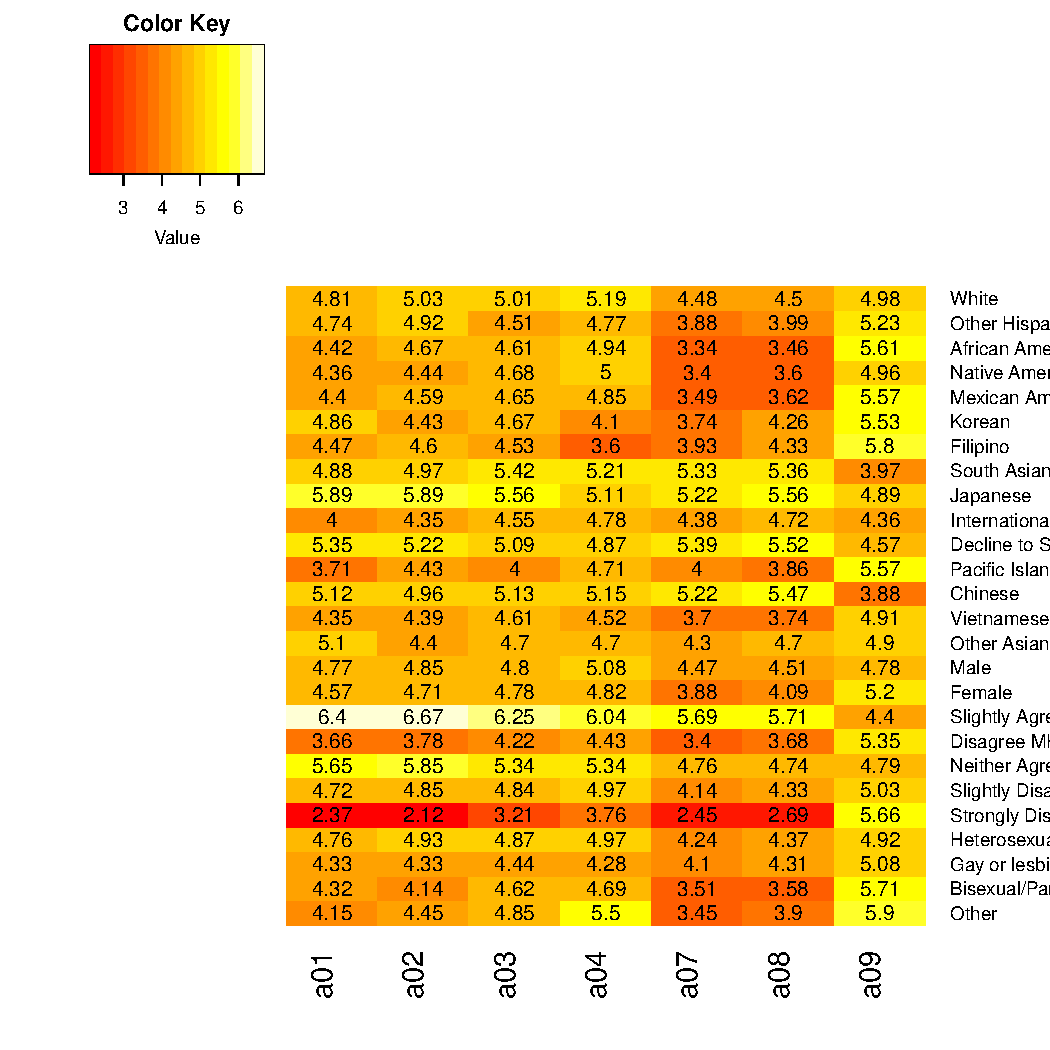
\includegraphics[width=\maxwidth]{figure/unnamed-chunk-18-1} 

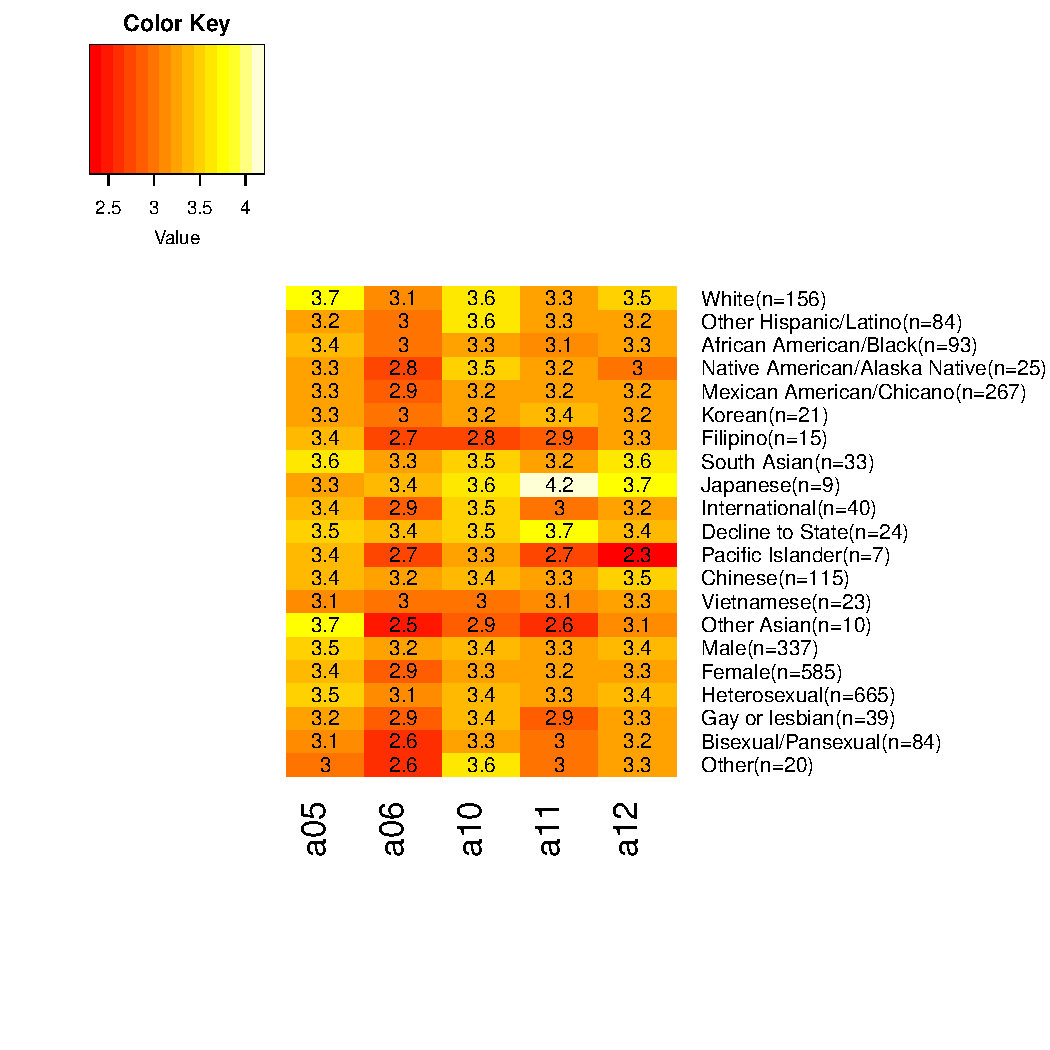
\includegraphics[width=\maxwidth]{figure/unnamed-chunk-18-2} 

\end{knitrout}

\end{document}
